\documentclass{oblivoir}
\usepackage{amsmath,amssymb,kotex,kswrapfig,mdframed,tabto,enumitem,graphicx}

%%% Counters
\newcounter{num}

%%% Commands
\newcommand\defi[1]
{\bigskip\par\noindent\stepcounter{num} \textbf{정의 \thenum) #1}\par\noindent}
\newcommand\theo[1]
{\bigskip\par\noindent\stepcounter{num} \textbf{정리 \thenum) #1}\par\noindent}
\newcommand\exam[1]
{\bigskip\par\noindent\stepcounter{num} \textbf{예시 \thenum) #1}\par\noindent}
\newcommand\prob[1]
{\bigskip\par\noindent\stepcounter{num} \textbf{문제 \thenum) #1}\par\noindent}

\newcommand\pb[1]{\ensuremath{\fbox{\phantom{#1}}}}

\newcommand\ba{\ensuremath{\:|\:}}

\newcommand\procedure[1]{\begin{mdframed}\vspace{#1\textheight}\end{mdframed}\bigskip}

\newcommand\an[1]{\bigskip\par\noindent\textbf{문제 #1)}\par\noindent}

%%% Meta Commands
\let\oldsection\section
\renewcommand\section{\clearpage\oldsection}

\let\emph\textsf

%%% Title
\title{미적분 1 : 04 연속함수}
\date{\today}
\author{}

\begin{document}
\maketitle

\tableofcontents
\clearpage

%%
\section{한 점에서의 연속}
\begin{mdframed}
%
\defi{}
함수 \(f(x)\)와 실수 \(a\)에 대하여,
\[f(a)=\lim_{x\to a}f(x)\]
가 성립하면
\begin{center}
함수 \(f(x)\)가 \(x=a\)에서 \emph{연속}이다
\end{center}
\noindent라고 말한다.
\end{mdframed}
\bigskip

따라서 다음 세 가지를 만족시켜야만 \(f(x)\)가 \(x=a\)에서 연속이다.
\begin{enumerate}
\item
\(f(a)\)가 존재한다.
\item
\(\displaystyle\lim_{x\to a}f(x)\)가 존재한다.
\item
\(\displaystyle f(a)=\lim_{x\to a}f(x)\)가 성립한다.
\end{enumerate}

%
\exam{}
\kswrapfig[Pos=r,Width=3cm]{exam_1}{
함수 \(f(x)=x+1\)와 실수 \(1\)에 대해
\begin{enumerate}
\item
\(f(1)\)이 존재한다(\(=2\)).
\item
\(\displaystyle\lim_{x\to 1}f(x)\)가 존재한다(\(=2\)).
\item
\(\displaystyle f(1)=\lim_{x\to 1}f(x)\)가 성립한다.
\end{enumerate}
따라서 \(f(x)\)는 \(x=1\)에서 연속이다.
}

\clearpage
%
\exam{}
\kswrapfig[Pos=r,Width=3cm]{exam_2}{
함수 \(g(x)=\begin{cases}x+1&(x<1)\\1&(x\ge1)\end{cases}\)와 실수 \(1\)에 대해
\begin{enumerate}
\item
\(g(1)\)이 존재한다(\(=2\)).
\item
\(\displaystyle\lim_{x\to 1}g(x)\)가 존재하지 않는다.\\
(좌극한과 우극한이 일치하지 않기 때문이다.)
\item
\(\displaystyle g(1)=\lim_{x\to 1}g(x)\)가 성립하지 않는다.
\end{enumerate}
따라서 \(g(x)\)는 \(x=1\)에서 연속이 아니다.
}

%
\prob{}
\kswrapfig[Pos=r,Width=3cm]{prob_1}{
함수 \(f(x)=x^2\)와 실수 \(1\)에 대해
\begin{enumerate}
\item
\(f(1)\)이 존재한다(\(=\pb{1}\)) / 존재하지 않는다.
\item
\(\displaystyle\lim_{x\to 1}f(x)\)가 존재한다(\(=\pb{1}\)) / 존재하지 않는다.
\item
\(\displaystyle f(1)=\lim_{x\to 1}f(x)\)가 성립한다 / 성립하지 않는다.
\end{enumerate}
따라서 \(f(x)\)는 \(x=1\)에서 연속이다 / 연속이 아니다.
}


%
\prob{}
\kswrapfig[Pos=r,Width=3cm]{prob_2}{
함수 \(\displaystyle g(x)=\frac{-x^2+2x}x\)와 실수 \(0\)에 대해
\begin{enumerate}
\item
\(g(0)\)이 존재한다(\(=\pb{1}\)) / 존재하지 않는다.
\item
\(\displaystyle\lim_{x\to 0}g(x)\)가 존재한다(\(=\pb{1}\)) / 존재하지 않는다.
\item
\(\displaystyle g(0)=\lim_{x\to 0}g(x)\)가 성립한다 / 성립하지 않는다.
\end{enumerate}
따라서 \(g(x)\)는 \(x=0\)에서 연속이다 / 연속이 아니다.
}

%
\prob{}
\kswrapfig[Pos=r,Width=3cm]{prob_3}{
함수 \(h(x)=\begin{cases}1&(x\neq1)\\3&(x=1)\end{cases}\)와 실수 \(1\)에 대해
\begin{enumerate}
\item
\(h(1)\)이 존재한다(\(=\pb{1}\)) / 존재하지 않는다.
\item
\(\displaystyle\lim_{x\to 1}h(x)\)가 존재한다(\(=\pb{1}\)) / 존재하지 않는다.
\item
\(\displaystyle h(1)=\lim_{x\to 1}h(x)\)가 성립한다 / 성립하지 않는다.
\end{enumerate}
따라서 \(h(x)\)는 \(x=1\)에서 연속이다 / 연속이 아니다.
}

%
\prob{}
다음 함수의 그래프를 그리고 연속성을 조사하여라.
\begin{enumerate}[label=(\arabic*)]
\item
\(y=|2x-2|\)는 \(x=1\)에서 연속이다 / 연속이 아니다.
\item
\(y=[x]\)는 \(x=0\)에서 연속이다 / 연속이 아니다.\\
(단, \([x]\)는 \(x\)를 넘지 않는 최대의 정수이다.)
\item
\(y=\displaystyle\frac{x^2-3x+2}{|x-2|}\)는 \(x=2\)에서 연속이다 / 연속이 아니다.
\end{enumerate}

\begin{figure*}[h!]
\centering
\noindent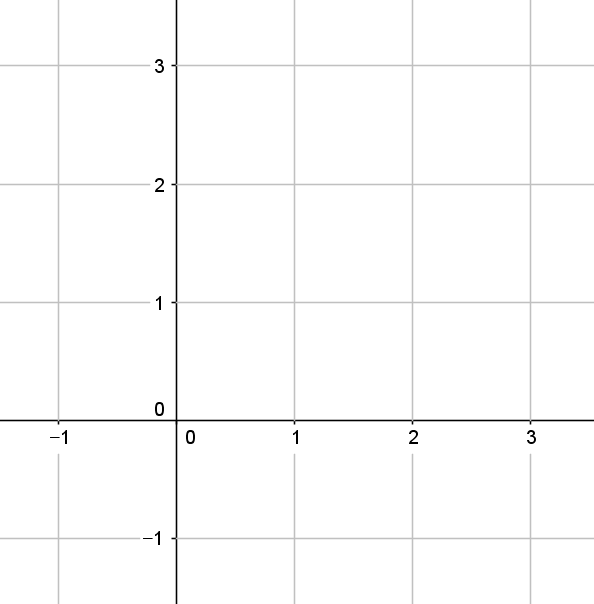
\includegraphics[width=0.3\textwidth]{-1_3}
~
\noindent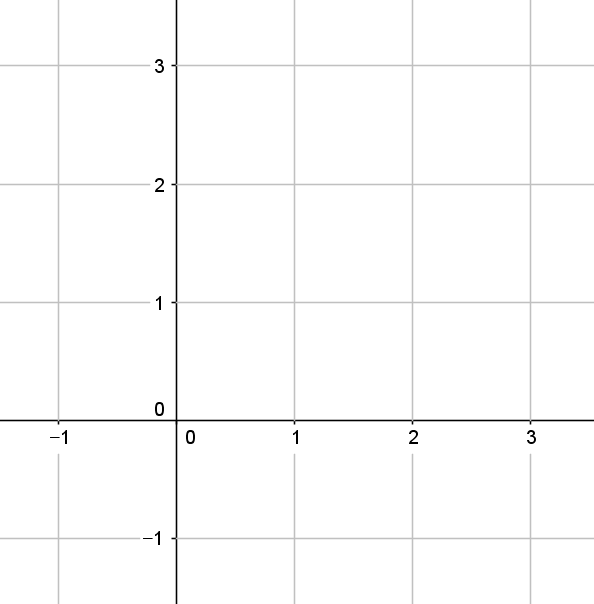
\includegraphics[width=0.3\textwidth]{-1_3}
~
\noindent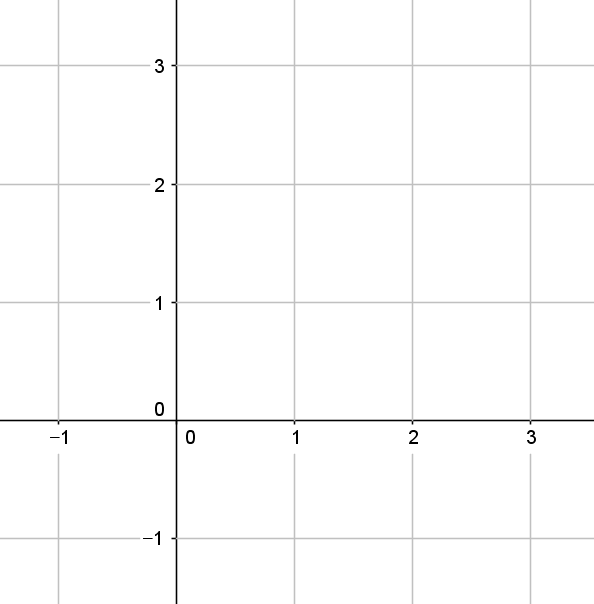
\includegraphics[width=0.3\textwidth]{-1_3}

\noindent
(1)\qquad\qquad\qquad\qquad\qquad(2)\qquad\qquad\qquad\qquad\qquad\qquad(3)
\end{figure*}

%%
\section{구간에서의 연속}
\begin{mdframed}
%
\defi{구간}
두 실수 \(a\), \(b\) (\(a<b\))에 대하여 다음과 같은 기호를 쓴다.
\begin{align*}
(a,b)&=\{x\ba a<x<b\}		\quad\cdots\cdots\quad\emph{열린 구간}\\
[a,b]&=\{x\ba a\le x\le b\}	\quad\cdots\cdots\quad\emph{닫힌 구간}\\
[a,b)&=\{x\ba a\le x<b\}\\
(a,b]&=\{x\ba a<x\le b\}
\end{align*}
\end{mdframed}
\bigskip

%
\exam{}
\begin{enumerate}[label=(\arabic*)]
\item
예를 들어, 열린 구간 \((1,3)\)은 집합 \(\{x\ba 1<x<3\}\)을 뜻한다.
또한, 닫힌구간 \([-2,2]\)는 집합 \(\{x\ba-2\le x\le 2\}\)를 뜻한다.
\begin{figure*}[h!]
\centering
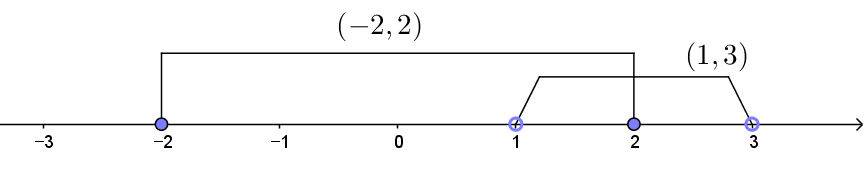
\includegraphics{intervals}
\end{figure*}
\item
\((2,5]\)이나 \([-3,\sqrt2)\)와 같이 한쪽이 닫혀있고, 한쪽은 열려있는 구간은 \emph{반열린구간}, 혹은 \emph{반닫힌 구간}이라고 불린다.
\item
\(\{x\ba x>2\}\)와 같은 집합은 \((2,\infty)\)와 같이 쓴다.
마찬가지로 \(\{x\ba x\le 5\}=(-\infty,5]\)가 성립하며, 실수 전체 집합은 \((-\infty,\infty)\)와 같이 쓰기도 한다.
\end{enumerate}

%
\prob{}
다음 부등식 혹은 등식의 해를 구간으로 나타내어라.
\begin{enumerate}[label=(\arabic*)]
\item
\(x^2-6x+5<0\)
\item
\(x^2-10x\le0\)
\item
\(2x+4\ge0\)
\item
\(x^2-2x+1=(x-1)^2\)
\end{enumerate}
\begin{mdframed}

%
\defi{}
함수 \(f(x)\)와 구간 \(I\)에 대하여, 구간 \(I\)의 모든 실수 \(a\)에 대해 함수 \(f(x)\)가 \(x=a\)에서 연속이면
\begin{center}
함수 \(f(x)\)가 구간 \(I\)에서 \emph{연속}이다
\end{center}
\noindent라고 말한다.
\end{mdframed}

%
\exam{}
\kswrapfig[Pos=r,Width=3cm]{exam_3}{
함수 \(f(x)=\begin{cases}-x+1&(x\le1)\\x&(x>1)\end{cases}\)에 대해
\begin{enumerate}[label=(\arabic*)]
\item
\(f(x)\)는 \((-1,0)\)에서 연속이다.
\(-1<a<0\)인 모든 실수 \(a\)에 대해 \(f(x)\)는 \(x=a\)에서 연속이기 때문이다.
\item
\(f(x)\)는 \([0,2]\)에서 연속이 아니다.
\(f(x)\)는 \(x=1\)에서 불연속이기 때문이다.
\end{enumerate}
}

%
\prob{}
구간 \([-1,9]\)에서 정의된 함수 \(f(x)\)의 그래프가 다음과 같이 주어질 때, 옳은 것을 모두 고르시오.
\vspace{-10pt}
\begin{figure*}[h!]
\centering
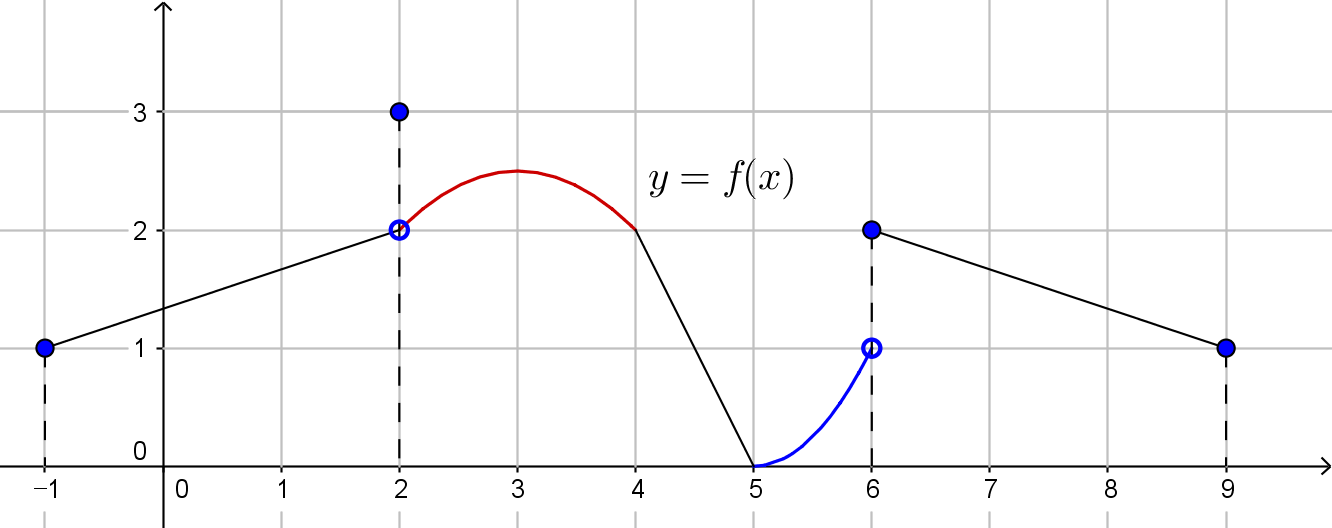
\includegraphics[width=0.8\textwidth]{prob_4}
\end{figure*}

\vspace{-10pt}
\begin{enumerate}
\item[ㄱ.]
\(\displaystyle\lim_{x\to2-}f(x)=\lim_{x\to2+}f(x)\)
\item[ㄴ.]
\(f(x)\)는 \(x=6\)에서 연속이다.
\item[ㄷ.]
\(f(x)\)는 \([3,5]\)에서 연속이다.
%\item
%\(f(x)\)는 \((5,8)\)에서 연속이다.
\item[ㄹ.]
불연속인 점은 \(3\)개이다.
\end{enumerate}

%
\prob{}
\(-2\le x<3\), \(3<x\le 6\)에서 정의된 함수 \(f(x)\)의 그래프가 다음과 같이 주어질 때, 옳은 것을 모두 고르시오.
\begin{figure*}[h!]
\centering
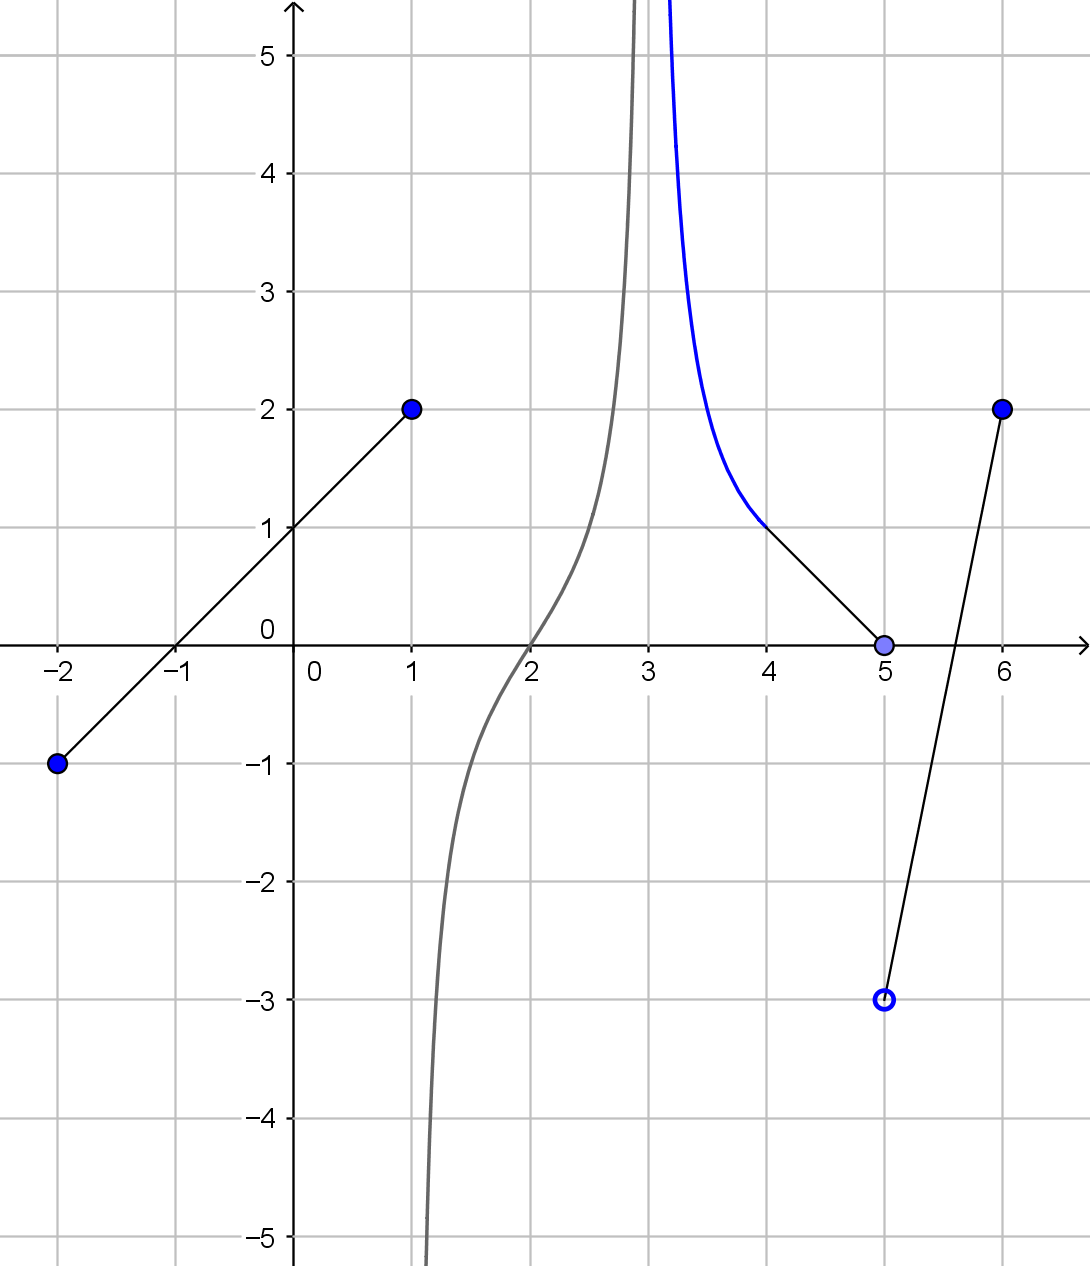
\includegraphics[width=0.8\textwidth]{prob_5}
\end{figure*}

\begin{enumerate}
%\item
%\(\displaystyle\lim_{x\to1-}f(x)=\lim_{x\to6-}f(x)\)
\item[ㄱ.]
\(f(x)\)는 \([4,6]\)에서 연속이다.
\item[ㄴ.]
\(\displaystyle\lim_{x\to3}f(x)=\infty\)
\item[ㄷ.]
\(f(x)\)는 \(x=3\)에서 연속이다.
\end{enumerate}

%%
\section{연속함수의 성질}

%
\exam{}
함수 \(f(x)\), \(g(x)\)가 \(x=a\)에서 연속일 때, 함수 \(f(x)+g(x)\)도 \(x=a\)에서 연속임을 증명하여라.
\begin{mdframed}
\(f(x)\)와 \(g(x)\)가 \(x=a\)에서 연속이므로,
\[\lim_{x\to a}f(x)=f(a),\qquad\lim_{x\to a}g(x)=g(a)\]
따라서
\begin{align*}
\lim_{x\to a}\{f(x)+g(x)\}
&=\lim_{x\to a}f(x)+\lim_{x\to a}g(x)\\
&=f(a)+g(a)
\end{align*}
이다.
그러므로 \(f(x)+g(x)\)는 \(x=a\)에서 연속이다.
\end{mdframed}
\bigskip

%
\prob{}
함수 \(f(x)\)가 \(x=a\)에서 연속일 때, \(kf(x)\)도 \(x=a\)에서 연속임을 증명하여라.
\procedure{0.3}

\clearpage
%
\prob{}
함수 \(f(x)\)와 \(g(x)\)가 \(x=a\)에서 연속일 때, \(f(x)g(x)\)도 \(x=a\)에서 연속임을 증명하여라.
\procedure{0.4}

일반적으로 다음 정리가 성립한다
\medskip

\begin{mdframed}
%
\theo{}
함수 \(f(x)\)와 \(g(x)\)가  \(x=a\)에서 연속이면 다음 함수들도 \(x=a\)에서 연속이다.
\begin{enumerate}[label=(\alph*)]
\item
\(kf(x)\)
\item
\(f(x)+g(x)\)
\item
\(f(x)-g(x)\)
\item
\(f(x)g(x)\)
\item
\(\displaystyle\frac{f(x)}{g(x)}\)\quad(단, \(g(x)\neq0\))
\end{enumerate}
\end{mdframed}
\bigskip

%%
\section{최대·최소의 정리와 사이값 정리}

%
\prob{}
다음 중 옳은 것을 모두 고르시오.
\begin{enumerate}
\item[ㄱ.]
닫힌 구간 \([0,3]\)에서  함수 \(f(x)=x^2-4x+5\)는 최댓값과 최솟값을 모두 가진다.
\item[ㄴ.]
열린 구간 \((2,4)\)에서 함수 \(g(x)=-2x+7\)의 최솟값을 가진다.
\item[ㄷ.]
닫힌구간 \([-2,2]\)에서 함수 \(h(x)=\begin{cases}x+2&(x<0)\\x-2&(x\ge0)\end{cases}\)는 최댓값과 최솟값을 모두 가진다.
\end{enumerate}

\begin{figure*}[h!]
\centering
\noindent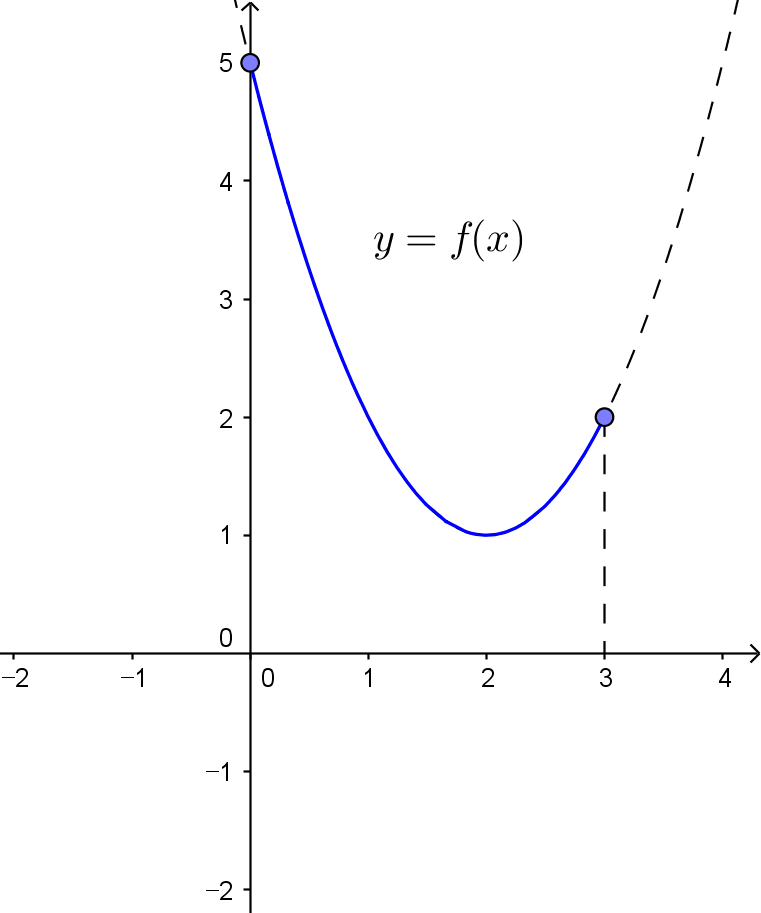
\includegraphics[width=0.3\textwidth]{maxmin_1}
~
\noindent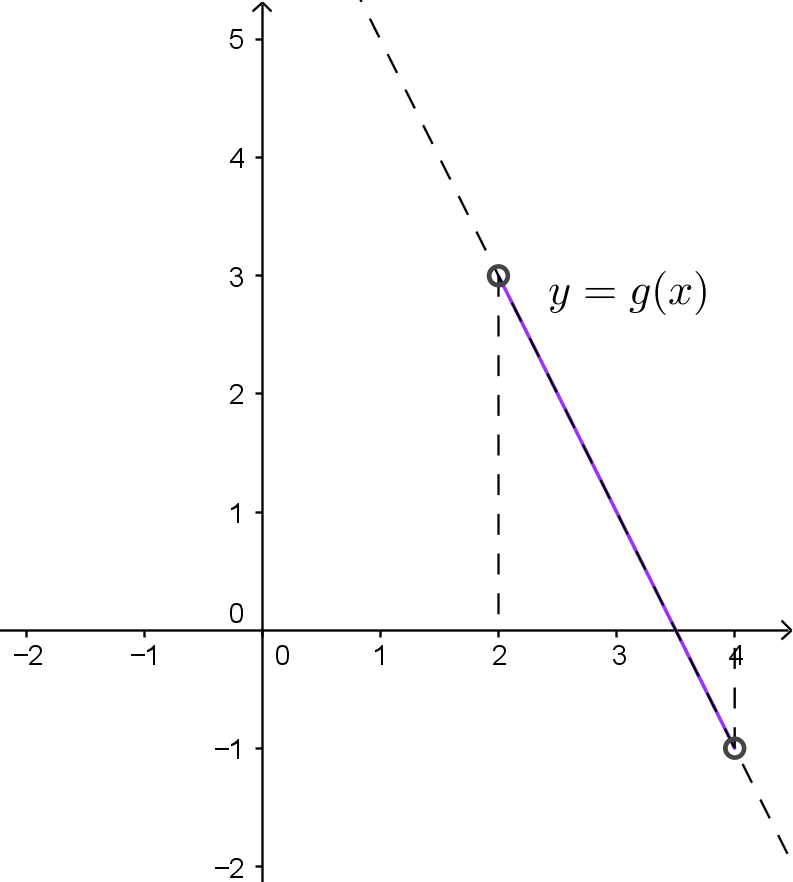
\includegraphics[width=0.3\textwidth]{maxmin_2}
~
\noindent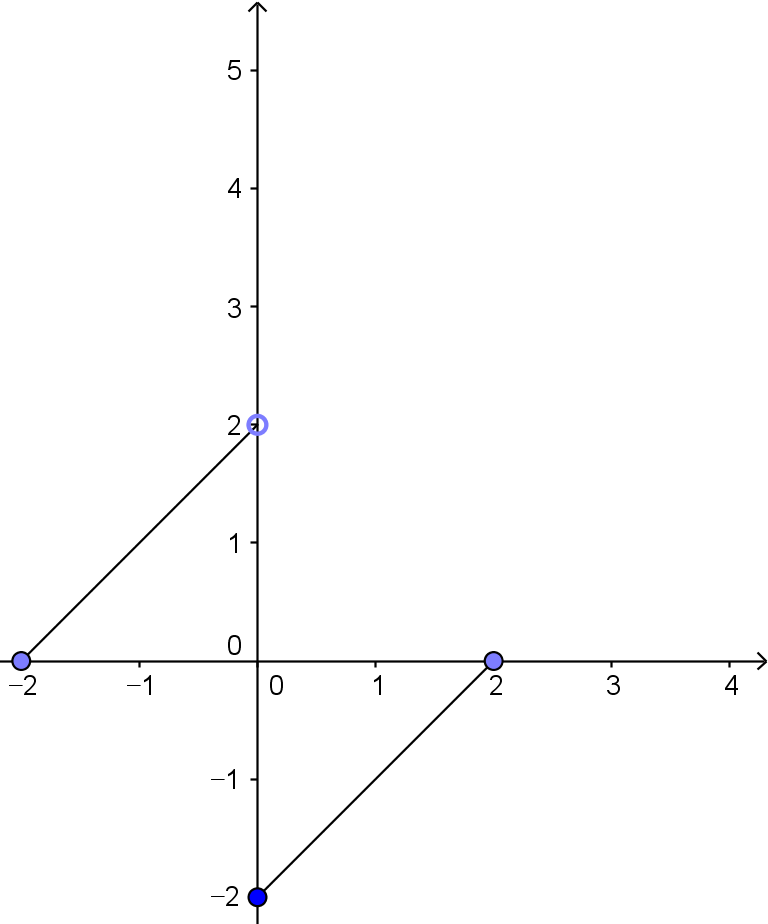
\includegraphics[width=0.3\textwidth]{maxmin_3}
\end{figure*}
\bigskip

연속함수의 최솟값과 최댓값에 대해서는 다음 정리가 성립한다.
\medskip

\begin{mdframed}
%
\theo{최대·최소의 정리}
함수 \(f(x)\)가 닫힌 구간 \([a,b]\)에서 연속이면 \(f(x)\)는 이 구간에서 최댓값과 최솟값을 가진다.
\end{mdframed}
\bigskip

\clearpage

%
\exam{}
연속 함수 \(f(x)\)가 \(f(1)=1\), \(f(4)=3\)를 만족한다고 하자.
\(y=f(x)\)의 그래프는 두 점 \(A(1,1)\), \(B(4,3)\)을 연속적으로 이은 선이므로 직선 \(y=2\)와 반드시 만나게 된다.
따라서 \(f(c)=2\)를 만족시키는 실수 \(c\)가 반드시 존재한다.

\begin{figure*}[h!]
\centering
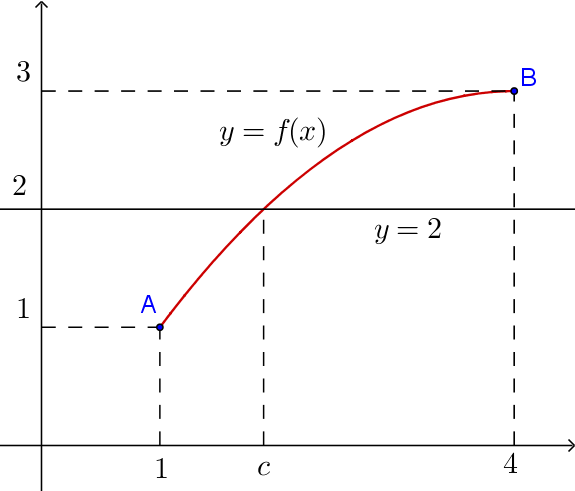
\includegraphics[width=0.5\textwidth]{intermediate_value}
\end{figure*}

일반적으로 다음 정리가 성립한다.
\medskip

\begin{mdframed}
%
\theo{사이값 정리}
함수 \(f(x)\)가 닫힌 구간 \([a,b]\)에서 연속이고 \(f(a)\neq f(b)\)이며, \(k\)가 \(f(a)\)와 \(f(b)\) 사이의 실수일 때,
\[f(c)=k\]
를 만족시키는 실수 \(c\)가 존재한다.
(단, \(a<c<b\))
\end{mdframed}
\bigskip

%
\prob{}
실수 전체에서 연속인 함수 \(f(x)\)에 대하여 \(f(-1)=1\), \(f(0)=3\), \(f(1)=-1\)일 때, 다음 물음에 답하여라.
\begin{enumerate}
\item[ㄱ.]
\(f(x)=-\frac12\)를 만족시키는 \(x\)가 적어도 하나 존재한다.
\item[ㄴ.]
\(f(x)=2\)를 만족시키는 \(x\)가 두 개 이상 존재한다.
\item[ㄷ.]
방정식 \(f(x)=0\)의 해가 적어도 하나 존재한다.
\end{enumerate}

%%
\section*{답}

%
\an{4}
존재한다, \(1\), 존재한다, \(1\), 성립한다, 연속이다.

%
\an{5}
존재하지 않는다, 존재한다, \(2\), 성립하지 않는다, 연속이 아니다.

%
\an{6}
존재한다, \(3\), 존재한다, \(1\), 성립하지 않는다, 연속이 아니다.

%
\an{7}
\begin{enumerate}[label=(\arabic*)]
\item
연속이다.
\item
연속이 아니다.
\item
연속이 아니다
\end{enumerate}

% 	
\an{10}
\begin{enumerate}[label=(\arabic*)]
\item
\((1,5)\)
\item
\([0,10]\)
\item
\([-2,\infty)\)
\item
\((-\infty,\infty)\)
\end{enumerate}

%
\an{13}
ㄱ, ㄷ.

%
\an{14}
ㄴ.

%
\an{19}
ㄱ.

%
\an{23}
ㄱ, ㄴ, ㄷ.

\end{document}